%%%%%%%%%%%%%%%%%%%%%%%%%%%%%%%%%%%%%%%%%%%%%%%%%%%%%%%%%%%%%%%%%%% 
%                                                                 %
%                            CHAPTER ONE                          %
%                                                                 %
%%%%%%%%%%%%%%%%%%%%%%%%%%%%%%%%%%%%%%%%%%%%%%%%%%%%%%%%%%%%%%%%%%% 
 
\chapter{INTRODUCTION}
In a social network with signed edges, positive edges
represent friendship while negative edges represent antagonism. An important problem
in the study of social networks is to understand the tension between these two forces~\cite{kleinberg-book}. Structural balance is a concept studying the influence of signed relationships on each other. The theory of structural balance has its origins in the work of Heider~\cite{Heider:46}. Cartwright and Harary then formalized Heider's idea and formulated the overall structure of a network with signed edges~\cite{Cartwright:56}. Davis~\cite{Davis:67} further gives a generalized theory by a relaxed balance assumption. In essence, structural balance theory considers certain configurations of positive and negative edges as socially and psychologically more plausible than others. In balance theory, a triangle, i.e. triad, is the smallest structural unit. It consists of three pairwise relationships between three people, and there are four distinct ways to label each relationship as positive or negative; see Figure~\ref{fig:balance_strong}
\begin{figure}[th]
\centering
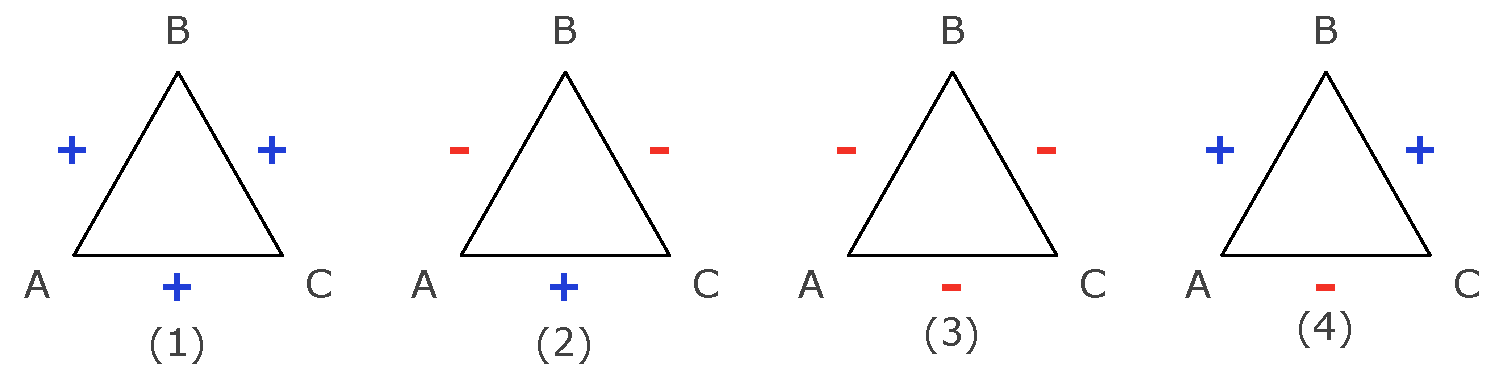
\includegraphics[width=4.8in]{Figs/strongBalance_hor.pdf}
\caption{\label{fig:balance_strong} Four different cases of triangular relationship.}
\end{figure}\\
It is argued that triads (1) (2) are more socially and psychologically reasonable than than triads (3) and (4)~\cite{Heider:46},~\cite{Cartwright:56}. The configurations of positive and negative relations in triads (3) (4) will bring tension that makes such triadic relationship unstable. Davis points out that the stress inside triad (4) is much more significant than it is in triad (3), and hence proposes a generalized balance theorem~\cite{Davis:67}. 

The structural balance theory provides a concise and elegant description of influence between interpersonal relationships. Moreover, it illustrates a nice connection between local configuration and global structural property in social networks. The key result of Cartwright-Harary's work is the structure theorem~\cite{Cartwright:56}: if a network is balanced, the nodes can be partitioned into two subsets such that all positive relationships are within subsets and all negative relationships are between subsets. Davis draws a similar theorem in the case when triad (3) in Figure~\ref{fig:balance_strong} is relaxed as balanced~\cite{Davis:67}. 

In recent research in online social networks, network balance plays a key role in many applications. One specific problem of interest is inferring new relationships and make recommendations based on existing relationships. We observe that the concept of structural balance is widely applied when developing algorithms for this type of prediction task. For example, Leskovec et al. generate a class of �triad features� in their prediction algorithm, i.e. a pair of relationships constraining a third relationship~\cite{Leskovec:2010}. They also use the structural balance as a touchstone to see the congruence between their practical results and the long studied theory. Another algorithm~\cite{golbeck:distrust2011} makes use of similar assumptions without explicit mention of balance theory in which trust and distrust relationships are mapped to metric distances on a continuous range. To some degree, the strong prediction performance of these algorithms justifies the structural balance theory. However, we will see the theory has its own weakness.
 
The arguments behind the balance theory imply a type of tendency towards balance for general social networks. That is, every social network will evolve to a state where every triad in it is balanced. The assumption by itself is congruent and intuitive; unstable triadic relationships (triads (3) (4) in Figure~\ref{fig:balance_strong}) will break and change to stable ones because of the inside tension. Regardless of other potential factors, a social network will inevitably reach a balanced state. As the ``balance process" is by nature a convergent process, every social network is expected to stay at a largely structurally balanced state. However, for most observed signed structures for social groups, exact structural balance does not hold~\cite{Doreian:02}. 

Despite the fact the structural balance theory is insufficient of empirical support, we regard the balance tendency a sound and natural description of social networks. In the physical world, an object stays at a state of minimum energy. Analogically, in social networks, does a triadic relationship stays at a state with minimum inner tension? We regard the structural balance theory as an incomplete description of balance in social networks. The current theory only deals with binary relationships while relationships in practice vary in degrees. While it is shown that strength is an important factor in many different social phenomena~\cite{Granovetter:1973}, the structural balance theory does not distinguish between relationships of the same sign but different strengths. In fact, when Cartwright and Harary first formalized the theory of structural balance, they also had the  following suggestions \cite{Cartwright:56}:

{\it ``...Obviously, however, many relationships of interest to psychologists(like liking, for example) exist in varying degrees. The fact means that our present use of graph theory can treat only the structural, and not the numerical, aspects of relations. While our treatment is thereby an incomplete representation of the strength of relations, we believe that conceptualization of the structural properties of relations is a necessary first step toward a more adequate treatment of the more complex situation." }

We take steps to analyze the social and psychological source of imbalance, and propose two fundamental principles regarding triadic balance in the general sense. Based on the principles, we establish an extended balance theory that deals with relationships with varying strengths. Heider's structural balance theory will be shown to be a special case under the generalized theory. 

In the second part of the thesis, we study the problem of social network convergence. The balance theory defines what is a  balanced state of a social network, but does not describe the dynamic aspect of the ``balance process". The problems of what each imbalanced triad will change to over time, and globally how an imbalanced network would evolve towards balance has not been studied in literature. It is plausible to have a decisive argument on whether triad (4) in Figure~\ref{fig:balance_strong} will change to triad (1) or triad (2), given the imperfect empirical evidence of structural balance itself. That is, if Bob's two friends Alice and Chris cannot get along with each other, whether Alice and Chris will resolve conflicts and become friends, or Bob teams up with one of them? In real life, questions like this really depend on how close Bob and Alice (Chris) is and how much conflict there is between Alice and Chris. For example, if the two friendships are very close while the conflict is subtle, we expect to see Alice and Chris become friends. On the contrary, if Bob is only close to Alice while the hatred between Alice and Chris is intense, it is likely that Bob will team up with Alice. With the extended balance theory, the problem becomes non-trivial and potentially solvable. We call such dynamic ``balance process" the {\bf social network convergence}. 

The convergence model helps complete the ``process" of network balance, as it models the principles of inter-relationship influence aspect of the network evolution. Due to its dynamic nature, the convergence model should inherit a predictive power over new relationships. For example, the strong triadic closure states that two people with a common close friend are very likely to friend each other in the future~\cite{Granovetter:1973}. We propose some famous predictive properties in social networks, such as ``two people with more common friends are more likely to become friends" as touchstones of the model, and show they hold under the convergence model. Both empirical experimental results and proofs are given.

To further justify our theory empirically, we use the convergence model to study the {\it edge sign prediction} problem. The {\it edge sign prediction} problem uses information of existing relationships to infer hidden relationships. To this date, many algorithms for this prediction problem are based on machine learning methods. These methods generate multiple structural features from the known relationships, and then use these features to classify the unknown relationships~\cite{Leskovec:2010},~\cite{golbeck:distrust2011},\cite{Guha:04}. We show why and how the convergence model can be applied in the prediction tasks over real online social network datasets. Our method consistently matches and outperforms the state of the art.

To summarize, we make the following
unique contributions in this thesis:
\begin{itemize}
\item We first introduce a new extended balance theory that allows
  arbitrary relationship strengths. We express balance with two
  simple principles that preserve the unique meaning of a
  positive, and a negative
  relationship. We show how balance can be reasoned when the strength of
  relationships are expressed as either discrete categorical values,
  as pairwise comparisons or as metric distances using the same two
  principles. Our method is novel, has sound social and psychological
  basis and captures the classical balance theory as a special case.
\item We propose a convergence model, describing how an imbalanced
  network evolves towards new balance. The assumption behind our model
  is that in resolving tensions within imbalanced relationships,
  people tend to avoid the effort of changing relationships if
  possible. The introduction of extended balance theory allows us to
  formulate the convergence problem of a social network as a Metric
  Multidimensional Scaling (MDS) optimization problem.
\item We show how the convergence model can be used to predict edge
  signs in social networks, and justify our theory through experiments
  on real datasets. Stress majorization is applied to solve
  MDS~\cite{Gansner:05}, and our method consistently matches and
  outperforms the state of the art. In addition, we show promising
  results towards providing solutions for the harder {\it link prediction
  problem}.
\end{itemize}
 Following the introduction, the thesis is organized as follows. Chapter 2 concisely reviews the structural balance theory and related work on {\it edge sign prediction} problem. Chapter 3 generalizes structural balance theory to allow relationships to have varying strengths, and establishes an extended balance theory to capture the general concept of balance. Chapter 4 discusses the social network convergence, and models it as an MDS problem. Some well-known social network phenomena are illustrated and proved under the convergence framework. Chapter 5 reviews the stress majorization technique to solve the MDS problem. Due to its high computational cost, two algorithms are introduced so that convergence model can be applied to large social networks. Chapter 6 examines the performance of the convergence model on the {\it edge sign prediction} problem. Chapter 7 concludes the thesis.

%%% Local Variables: 
%%% mode: latex
%%% TeX-master: t
%%% End: 
